%!TEX root=../oi-magistr-si.tex
\section[AOS - Kompozice služeb]{Webové služby, automatická kompozice služeb. Orchestrace a choreografie, web mash-up. Modelování služeb a procesů (BPMN, BPEL).}

Na kompozitní službu se můžeme dívat jako na sadu služeb, které spolu spolupracují za účelem vykonání určitého procesu, který definuje interakční workflow. \textbf{Orchestrace} a \textbf{choreografie} jsou rozdílné vzory pro vytváření kompozice služeb. Jazyky pro popis vykonávaného procesu (a tedy i pro popis spolupráce služeb) jsou např. BPMN, BPEL, UML.

\subsection{Orchestrace}
Při tomto přístupu je centrální prvek, který koordinuje všechny zapojené služby. Tento centrální prvek může být také webová služba. Zúčastněné služby nevědí, a ani nemusí vědět, že jsou účastníky nějakého většího procesu, o tom ví jen centrální prvek. Iterakce při orchestraci nastávají na úrovni zpráv.

\subsection{Choreografie}
U choreografie není centrální prvek procesu, a proto všechny zapojené služby ví, kdy volat a s kým dalším spolupracovat.

V praxi se více využívá orchestrace, protože se díky centrálnímu prvku lépe zotavuje z chyb (chyby jsou odchytávány na jednom místě).

\subsection{Mashup}
Aplikace kombinující data/funkcionalitu z 2 a více zdrojů.

\begin{itemize}[itemsep=0px]
\item Client-based - všechny data se z více služeb volají z klientova prohlížeče (problém s javascriptem Same-Origin Security Policy - POST dotazy).
\item Server-based - Prostředník v podobě serveru, uživatel se dotazuje na jeden server, a ten za něj získává data z ostatních služeb.
\end{itemize}

\subsection{Modelovací jazyky BPMN, BPEL}

\paragraph{BPMN (Business process modeling notation)} Grafická reprezentace pro specifikaci byznys procesu. Podobné UML. Poskytuje mapování mezi grafickou notací a BPEL.

\begin{figure}[h!]
\centering
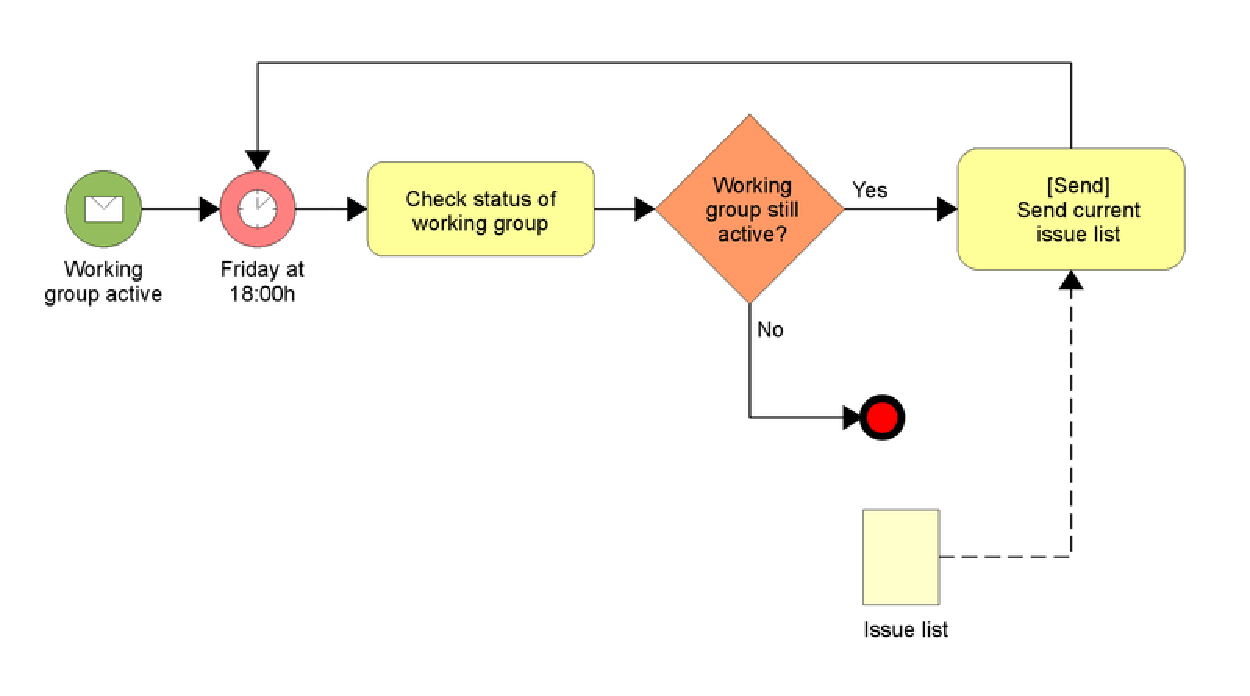
\includegraphics[width=100mm]{11/images/bpmn}
\end{figure}

\paragraph{BPEL} Business Process Execution Language je jazyk pro popis WS kompozice. Základ toho jazyka tvoří WSFL a XLANG. WSFL je zkratka pro Web Services Flow Language, jazyk vytvořený IBM pro popis kompozice webových služeb. XLANG je rozšíření WSDL. Zjednodušeně se dá říct, že popis služby v XLANG se skládá z popisu dané služby ve WSDL a popisu chování služby jako části byznys procesu. Varianta BPEL pro webové služby se označuje BPEL4WS (někdy také WS-BPEL). Tento jazyk rozšiřuje základní interakční schéma mezi službami o podporu byznys transakcí.

Je to programovací jazyk v XML?

BPMN --> BPEL --> Application